\documentclass[10pt]{beamer}
\usepackage{beamerthemesplit} % new 
\usepackage{media9}
\usepackage{multimedia}
\usepackage{tcolorbox}
\usepackage{hyperref}
\usepackage{tikz}
\usepackage{pgfplots}
\usepackage{graphicx}
\usetheme{Frankfurt}
%\usetheme{Madrid}
%\usetheme{Copenhagen}

%Document begins
\begin{document}
\title{\textcolor{green}{M}usic, \textcolor{green}{M}achine And \textcolor{green}{M}athematics} 
\author{\textbf{\textcolor{green}{M}annan, \textcolor{green}{M}ajhi}}
%\date{\today} 
\date{\textcolor{green}{M}arch 24, 2015}
\frame{\titlepage} 

\frame{\frametitle{Overview}\tableofcontents} 


\section{Storing And Reproducing Sound}
\begin{frame}
\frametitle{Computer Generation of Sound}
\begin{block}{What is Sound on a computer?}

\begin{tikzpicture}[domain =0:6.14, scale = 0.5]
\draw[thick,color=black, ->] (0,0)-- (6.14,0);
\draw[thick, color=black, <->] (0,-1) -- (0,1);
\draw [red] plot  (\x,{sin(\x r)});

\draw[thick,color=black, ->] (14,0)-- (14+6.14,0);
\draw[thick, color=black, <->] (14,-1) -- (14,1);
%\filldraw circle (6,0) (2 pt);
\foreach \i in {1,...,7}{
\pgfmathsetmacro{\y}{sin((\i-1) r)}

\filldraw[red] (14+\i-1,\y) circle (2 pt);

}
\node[draw, rectangle, anchor = west] at (10,0) {$\Large \rightarrow$};
\end{tikzpicture}


\end{block}


\begin{block}{Then to a speaker}
\begin{tikzpicture}[domain =0:6.14, scale = 0.5]
\draw[thick,color=black, ->] (0,0)-- (6.14,0);
\draw[thick, color=black, <->] (0,-1) -- (0,1);
\foreach \i in {1,...,7}{
\pgfmathsetmacro{\y}{sin((\i-1) r)}

\filldraw[red] (\i-1,\y) circle (2 pt);

}
\node[draw, rectangle, anchor = west] at (10,0) {$\Large \rightarrow$};
\node[anchor = west] at (14,0) {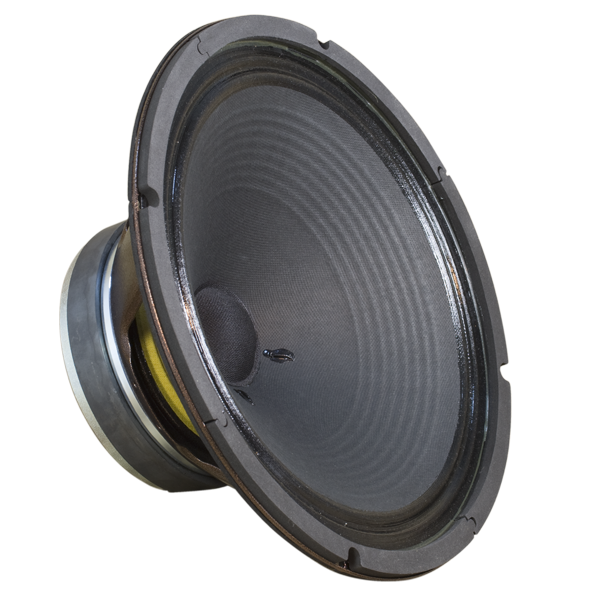
\includegraphics[width = 0.25\textwidth]{speaker.png}};
\end{tikzpicture}


\end{block}
\end{frame}


\begin{frame}
\frametitle{How to choose the sampling rate}
\begin{block}{Sampling rate = discretization}
That is to say, the sampling rate has the same issues as discretization choices do in numerical mathematics. How can the necessary information be captured most efficiently?
\end{block}

\begin{block}{CDs}
CDs use 44.1 kHz sampling. Why?
\end{block}
\end{frame}

\begin{frame}
\frametitle{Capturing a pressure wave}
\begin{block}{Sampling at 1.75 of the period}
\begin{tikzpicture}[domain =0:50, scale = 0.25, samples = 100]
\draw [red] plot  (\x,{sin(\x r)});
\foreach \i in {1,...,6}{
\pgfmathsetmacro{\x}{3.14*2*(1.75)*(\i-1)}
\pgfmathsetmacro{\y}{sin(\x r)}
\filldraw[black] (\x,\y) circle (3 pt);
}
\end{tikzpicture}
\end{block}

\begin{block}{Sampling at 0.75 of the period}
\begin{tikzpicture}[domain =0:50, scale = 0.25, samples = 100]
\draw [red] plot  (\x,{sin(\x r)});
\foreach \i in {1,...,10}{
\pgfmathsetmacro{\x}{3.14*2*(0.75)*(\i-1)}
\pgfmathsetmacro{\y}{sin(\x r)}
\filldraw[black] (\x,\y) circle (2 pt);
}
\end{tikzpicture}
\end{block}

\begin{block}{Sampling at 0.45 of the period}
\begin{tikzpicture}[domain =0:50, scale = 0.25, samples = 100]
\draw [red] plot  (\x,{sin(\x r)});
\foreach \i in {1,...,25}{
\pgfmathsetmacro{\x}{3.14*2*(0.45)*(\i-1)}
\pgfmathsetmacro{\y}{sin(\x r)}
\filldraw[black] (\x,\y) circle (2 pt);
}
\end{tikzpicture}
\end{block}
\end{frame}

\begin{frame}
\frametitle{Nyquist}

\begin{block}{Nyquist-Shannon Theorem}
If a function $Q$ is composed of continuous periodic waves (i.e. a nice fourier series) and has a highest frequency component in hertz  $f_{max}$ then the data of a sampling rate of at least $2f_{max}$ can be used to exactly determine $Q$.
\end{block}

\end{frame}


\section{Music With Machine}
\begin{frame}
 Pd Examples
 \end{frame}
 

\begin{frame}
\frametitle{How Can 2 Sound Waves Interact?}
\begin{block}{First, what happens when two sound waves meet?}
They add.
\end{block}

\end{frame}

\begin{frame}
\frametitle{The math of 2 wave friends}
\begin{block}{Wave$_1$ \& Wave$_2$}
Suppose Wave$_1 = A\cos(wt + k)$ and Wave$_2 = A\cos(w't + k')$. Then,
\begin{align*}
W_1 + W_2 =&A\cos(wt + k) + A\cos(w't + k')\\
=&2A\cos(\frac{(w+w')t+(k+k')}{2})\cos(\frac{(w-w')t +(k- k')}{2})
\end{align*}
\end{block}

\end{frame}

\begin{frame}
\frametitle{Aural Beating}
\begin{block}{The math of the given example}
Suppose Wave$_1 = \cos(440t)$ and Wave$_2 = \cos(435t)$. Then,
\begin{align*}
W_1 + W_2 =&\cos(440t) + \cos(435t)\\
=&2\cos(\frac{875t}{2})\cos(\frac{5t}{2})
\end{align*}
\end{block}

\begin{block}{}
\center 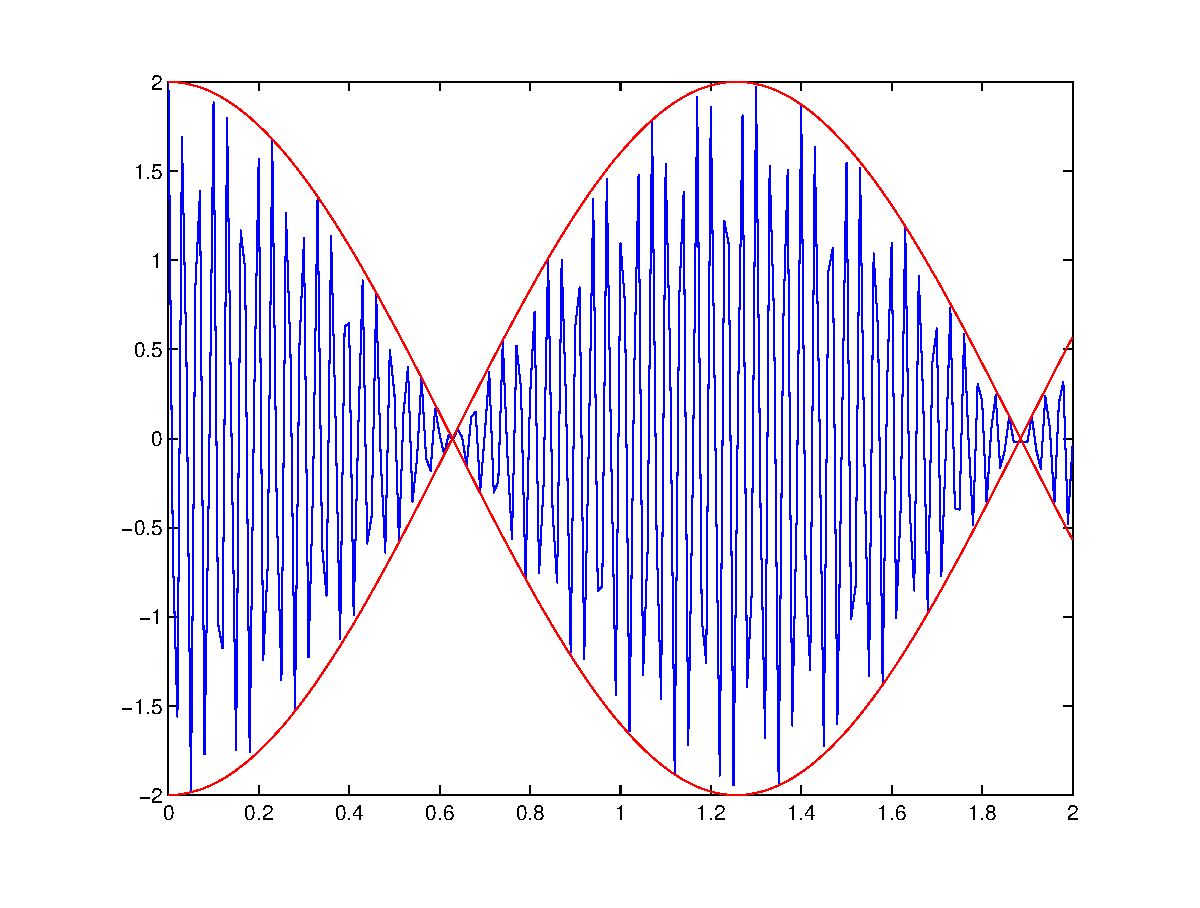
\includegraphics[width = 0.5\textwidth]{BeatingWave.eps}
\end{block}


\end{frame}

\begin{frame}
\frametitle{Computer Generation of Sound}
\begin{block}{What is Sound on a computer?}

\begin{tikzpicture}[domain =0:6.14, scale = 0.5]
\draw[thick,color=black, ->] (0,0)-- (6.14,0);
\draw[thick, color=black, <->] (0,-1) -- (0,1);
\draw [red] plot  (\x,{sin(\x r)});

\draw[thick,color=black, ->] (14,0)-- (14+6.14,0);
\draw[thick, color=black, <->] (14,-1) -- (14,1);
%\filldraw circle (6,0) (2 pt);
\foreach \i in {1,...,7}{
\pgfmathsetmacro{\y}{sin((\i-1) r)}

\filldraw[red] (14+\i-1,\y) circle (2 pt);

}
\node[draw, rectangle, anchor = west] at (10,0) {$\Large \rightarrow$};
\end{tikzpicture}


\end{block}


\begin{block}{Then to a speaker}
\begin{tikzpicture}[domain =0:6.14, scale = 0.5]
\draw[thick,color=black, ->] (0,0)-- (6.14,0);
\draw[thick, color=black, <->] (0,-1) -- (0,1);
\foreach \i in {1,...,7}{
\pgfmathsetmacro{\y}{sin((\i-1) r)}

\filldraw[red] (\i-1,\y) circle (2 pt);

}
\node[draw, rectangle, anchor = west] at (10,0) {$\Large \rightarrow$};
\node[anchor = west] at (14,0) {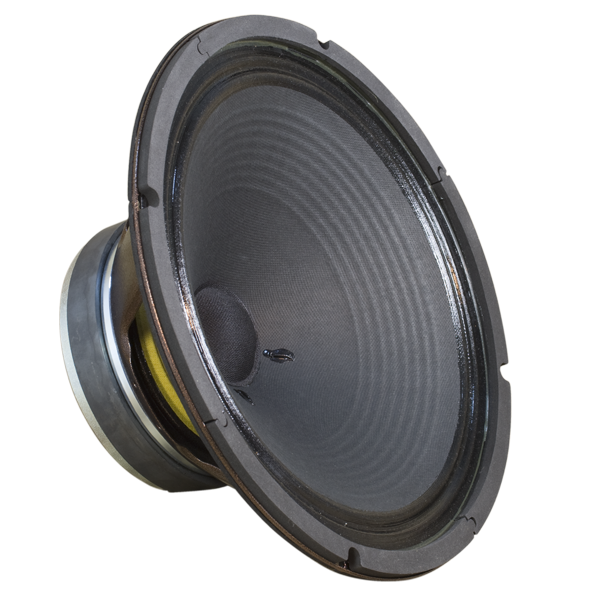
\includegraphics[width = 0.25\textwidth]{speaker.png}};
\end{tikzpicture}


\end{block}
\end{frame}

\begin{frame}
\begin{block}{Sampling at $\Delta t$}
\begin{tikzpicture}[domain =0:6.14, scale = 0.5]
\draw[thick,color=black, ->] (0,0)-- (6.14,0);
\draw [red] plot  (\x,{sin(\x r)});
\foreach \i in {1,...,7}{
\pgfmathsetmacro{\y}{sin((\i-1) r)}

\filldraw[red] (\i-1,\y) circle (2 pt);

}
\end{tikzpicture}
\end{block}

\begin{block}{Sampling at $2\pi+\Delta t$}
\begin{tikzpicture}[domain =0:30, scale = 0.4, samples = 100]
\draw[thick,color=black, ->] (0,0)-- (6.14,0);
\draw [red] plot  (\x,{sin(\x r)});
\foreach \i in {1,...,7}{
\pgfmathsetmacro{\x}{ 6.28*(\i-1)+(\i-1)}
\pgfmathsetmacro{\y}{sin( \x r)}

\filldraw[red] (\x,\y) circle (2.5 pt);

}

\end{tikzpicture}
\end{block}


\end{frame}

\section{Pure SineWaves Are Not Natural}

\begin{frame}
\frametitle{Sounds from instruments}

\begin{block}{Fundamental and overtones}
\center 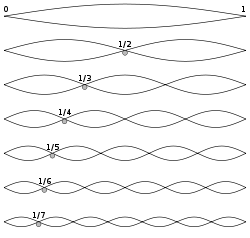
\includegraphics[scale = 0.75]{Harmonics.png};
\end{block}

\end{frame}



\end{document}